\section{Problem Description and Analysis}
%
% SUBSECTION %
%
\subsection{Problem description}\label{sec:problemDescription}
The need for secure telecommunications is required for electronic commerce and internet pricacy. Security requirements include confidentiality, authentication, data integrity and non-repudiation. 
These services are offered by public key cryptosystems, and the most popular of which is the RSA encryption scheme.
The fundamental operation of the algorithm is modular exponentiation which is achieved by repeated modular multiplications. 
With high bit lengths required to provide adequate security the need for specialized hardware to provide high enough throughput is preferred. 
There are many algorithms with different grades of efficiency to solve this problem and some of them will be discussed in this paper.
The RSA algorithm was invented by Rivest, Shamir and Adleman in 1977. 

Suppose Alice wishes to send a secret message to Bob. 
In a secret key system, Alice and Bob need to know the same secret key and so it must be communicated via some secure channel. 
In a public key system, Bob broadcasts his public key, and Alice can use it to encode a message. 
The design of the cryptosystem is such that only Bob can decode the encrypted message, but no exchange of secret keys is necessary. 

The algorithm consists of 5 parameters; $n$,$p$,$q$,$e$ and $d$. 
$p$ and $q$ are two random large prime numbers, and $n$ can be calculated by multiplying 
them together, $n=pq$. $e$ is the public exponent and has to be in the range $1<e<\phi(n)$ 
such that $gcd(e,\phi(n))=1$. $\phi(n)$ is Euler's totient function of n, given by
%
\begin{equation}
    \phi(n)=(p-1)(q-1)
\end{equation}
%
The private exponent, $d$, is obtained by inverting $e$ $modulo$ $\phi(n)$, i.e
%
\begin{equation}
    d=e^{-1}\mod{\phi(n)}
\end{equation}
%
In practice, $e$, is often chosen to be a small number which reduces the amount of computation needed to perform encryption. The strength of RSA depends on the key size, $k$, and the number of bits in $n$. Breaking RSA is believed to be as hard as factorizing $n$ to $p$,$q$, which is extremely time consuming with the current technology and fairly large key sizes. 
%
In the RSA cryptosystem, Alice must first find Bob's public key ($n$, $e$) which are the modulus and the exponent, respectively. She calculates the ciphertext, $C$, from the plaintext, $P$, by: 
%
\begin{equation}
    C=P^e\mod{n}
\end{equation}
%
where P is the plaintext such that $0<=P<=n$. To decode the message, Bob uses his private key ($n$,$d$) to recover the plaintext, $P$, from the ciphertext,$C$, by:
%
\begin{equation}
    P=C^d\mod{n}
\end{equation}
%
The problem with implementing this in hardware on an FPGA is that the exponential multiplication
$M^k$ can be very computational heavy, depending on the chosen algorithm. In \cref{sec:differentAlternatives} different algorithms and solutions will be presented.
%
% SUBSECTION
\newpage
\subsection{Requirements}
%
The RSA encryption/decryption circuit is to meet the following requirements:
%
\begin{itemize}
    \item The design must implement the RSA encryption algorithm.
    \item Encrypt/decrypt a message of length 128 bits as fast as possible.
    \item The target frequency is 50 MHz.
    \item The design must use less than 50 \% of the resources in a
        \emph{Xilinx Zynq\textregistered-7000} device.
    \item The design entity declaration must match the entity given in \cref{listing:RSAcore_entity}.
    \item The design must implement the interface in \cref{fig:interface_protocol}
\end{itemize}
%
\begin{lstlisting}[caption=Entity declaration, label=listing:RSAcore_entity]
entity RSACore is
    port (
        Clk          : in std_logic;
        Resetn       : in std_logic;
        InitRsa      : in std_logic;
        StartRsa     : in std_logic;
        DataIn       : in std_logic_vector(31 downto 0);
        DataOut      : out std_logic_vector(31 downto 0);
        CoreFinished : out std_logic
    );
end RSACore;
\end{lstlisting}
%
\begin{figure}[htp]
    \centering
    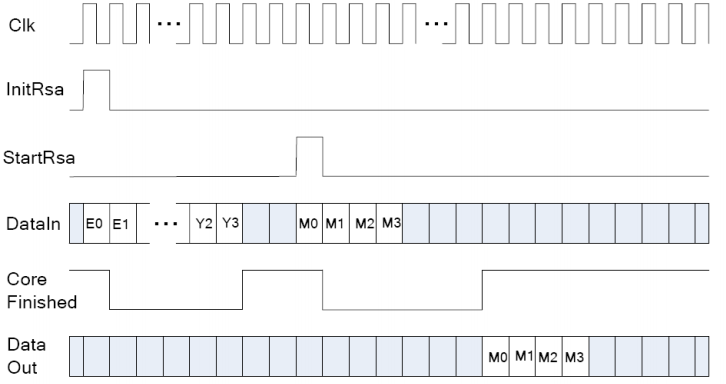
\includegraphics[width=0.7\textwidth]{images/interface_protocol}
    \caption{The interface protocol for the RSA encryption circuit}
    \label{fig:interface_protocol}
\end{figure}
%
% SUBSECTION
%
%\subsection{Discussion and further investigation}
%What do we need to investigate further before proposing a solution?


%\todo[inline]{Describe the FPGA}
%\todo[inline]{Describe the rsa algorithm (history and math)}
%\todo[inline]{Many ways to implement it on hardware}
%\todo[inline]{Describe montgogemry in math and some bla,bla about the algorithm}
%\todo[inline]{What is the strengths of doing this.}
%\todo[inline]{Main requirements. How fast do we need it to be? How many bits etc.}
%\todo[inline]{Investigate further. python model. reading other papers etc.}
